\documentclass[tikz,border=8pt]{standalone}
\usepackage{amsmath}
\usetikzlibrary{arrows.meta,calc}
\definecolor{ink}{HTML}{21352F}
\definecolor{teal}{HTML}{087F7B}
\definecolor{blue}{HTML}{4B77A8}
\definecolor{gold}{HTML}{C58B2A}
\begin{document}
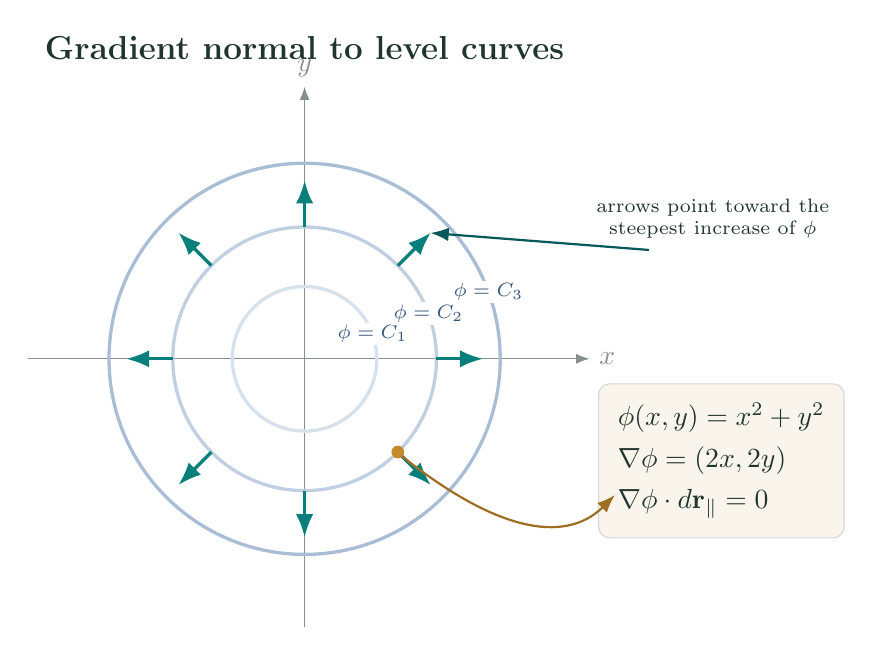
\begin{tikzpicture}[font=\sffamily,text=ink,>=Latex,scale=1.08]
  \node[font=\bfseries\large] at (0,3.65)
    {Gradient normal to level curves};
  \draw[->,ink!55] (-3.25,0)--(3.35,0) node[right] {$x$};
  \draw[->,ink!55] (0,-3.15)--(0,3.2) node[above] {$y$};
  \foreach \r/\c in {0.85/22,1.55/35,2.30/48}{
    \draw[blue!\c,very thick] (0,0) circle (\r);
  }
  \node[fill=white,inner sep=1pt,font=\scriptsize,text=blue!75!black]
    at ({0.85*cos(20)},{0.85*sin(20)}) {$\phi=C_1$};
  \node[fill=white,inner sep=1pt,font=\scriptsize,text=blue!75!black]
    at ({1.55*cos(20)},{1.55*sin(20)}) {$\phi=C_2$};
  \node[fill=white,inner sep=1pt,font=\scriptsize,text=blue!75!black]
    at ({2.30*cos(20)},{2.30*sin(20)}) {$\phi=C_3$};
  \foreach \a in {0,45,...,315}{
    \coordinate (P) at ({1.55*cos(\a)},{1.55*sin(\a)});
    \coordinate (Q) at ({2.10*cos(\a)},{2.10*sin(\a)});
    \draw[teal,very thick,->] (P)--(Q);
  }
  \fill[gold] ({1.55*cos(-45)},{1.55*sin(-45)}) circle (0.075);
  \node[align=left,draw=ink!20,fill=gold!9,rounded corners=4pt,
        inner sep=7pt] at (4.9,-1.2)
    {$\phi(x,y)=x^2+y^2$\\[3pt]
     $\nabla\phi=(2x,2y)$\\[3pt]
     $\nabla\phi\cdot d\mathbf r_{\parallel}=0$};
  \draw[gold!80!black,thick,->]
    ({1.55*cos(-45)+0.05},{1.55*sin(-45)-0.05})
    .. controls (2.6,-2.3) and (3.25,-2.0) .. (3.65,-1.6);
  \node[font=\scriptsize,align=center] at (4.8,1.65)
    {arrows point toward the\\steepest increase of $\phi$};
  \draw[teal!70!black,thick,->] (4.05,1.28)--(1.48,1.48);
\end{tikzpicture}
\end{document}
